\documentclass[11pt,a4paper]{article}

\usepackage[T1]{fontenc}
\usepackage[utf8]{inputenc}
\usepackage[brazil]{babel}
\usepackage{amsmath,amssymb}
\usepackage[top=2.5cm,bottom=2.5cm,left=2.6cm,right=2.6cm]{geometry}
\usepackage{graphicx}
\usepackage{booktabs}
\usepackage{listings}
\usepackage{xcolor}
\usepackage[hidelinks]{hyperref}
\usepackage{caption}
\usepackage{fancyhdr}
\usepackage{enumitem}
\usepackage{titlesec}
\usepackage{float}

\definecolor{azul}{HTML}{1F3864}
\definecolor{cinza}{HTML}{52514E}
\definecolor{fundocod}{HTML}{F7F7F5}

\newcommand{\repositorio}{https://github.com/vkmatsu/An-lise-de-Algoritmos-Aplicada-ao-Cadastro-de-Bolsistas-da-CAPES}

\titleformat{\section}{\normalfont\Large\bfseries\color{azul}}{\thesection}{0.6em}{}
\titleformat{\subsection}{\normalfont\large\bfseries\color{azul}}{\thesubsection}{0.6em}{}

\captionsetup{font=small,labelfont={small,bf},textfont=it}

\pagestyle{fancy}
\fancyhf{}
\fancyfoot[C]{\small\color{cinza}\thepage}
\renewcommand{\headrulewidth}{0pt}

\lstdefinestyle{c}{
  language=C,
  basicstyle=\ttfamily\scriptsize,
  keywordstyle=\color{azul},
  commentstyle=\color{cinza}\itshape,
  stringstyle=\color{black!70},
  numbers=left,
  numberstyle=\tiny\color{cinza},
  numbersep=8pt,
  backgroundcolor=\color{fundocod},
  frame=single,
  rulecolor=\color{black!15},
  breaklines=true,
  showstringspaces=false,
  tabsize=4,
  columns=fullflexible,
  keepspaces=true,
}

\lstdefinestyle{terminal}{
  basicstyle=\ttfamily\scriptsize,
  backgroundcolor=\color{fundocod},
  frame=single,
  rulecolor=\color{black!15},
  breaklines=true,
  columns=fullflexible,
  keepspaces=true,
}

\begin{document}

% ------------------------------------------------------------------ capa
\begin{titlepage}
\centering
\vspace*{3cm}
{\color{azul}\Huge\bfseries Análise de Algoritmos Aplicada ao\\[0.3cm] Cadastro de Bolsistas da CAPES\par}
\vspace{1cm}
{\large\color{cinza} Importação de registros sem redundância por busca sequencial:\\ análise teórica, demonstração por indução e validação experimental\par}
\vspace{3cm}
{\large Aluno: \underline{\hspace{6cm}}\par}
\vspace{0.6cm}
{\large Disciplina: \underline{\hspace{5.4cm}}\par}
\vspace{0.6cm}
{\large Professor: \underline{\hspace{5.6cm}}\par}
\vspace{2.5cm}
{\large\bfseries Repositório Git público\par}
\vspace{0.3cm}
{\ttfamily\small \url{\repositorio}\par}
\vfill
{\color{cinza} Setembro de 2026\par}
\end{titlepage}

\tableofcontents
\newpage

% ------------------------------------------------------------------ 1
\section{Introdução}

A CAPES mantém um serviço que recebe solicitações de cadastro de bolsistas por meio de uma API. Essas solicitações chegam em arquivos CSV e precisam ser incorporadas a um cadastro principal sem que se criem registros duplicados. O problema é, portanto, de deduplicação em fluxo: para cada registro recebido é preciso decidir se o nome já consta no cadastro de destino antes de copiá-lo.

Este trabalho implementa esse serviço em linguagem C e, sobretudo, analisa rigorosamente o custo do algoritmo empregado. A verificação de redundância é feita por \textbf{busca sequencial} sobre os nomes já presentes no destino, e o programa foi instrumentado com um contador do número de comparações entre nomes realizadas durante a execução.

O objetivo central não é apenas demonstrar que o programa funciona, mas confrontar uma previsão teórica com evidências medidas. A análise parte de dois parâmetros: $Q$, a quantidade de cadastros já existentes no arquivo de destino no início da execução, e $N$, a quantidade de nomes novos e distintos a inserir. A função de custo deduzida é

\begin{equation}
T(N, Q) \;=\; N \cdot Q \;+\; \frac{N(N-1)}{2},
\label{eq:modelo}
\end{equation}

\noindent que é demonstrada formalmente por indução matemática e depois submetida a validação experimental. Os experimentos foram conduzidos sobre o arquivo \texttt{bolsistas-2025.csv}, que contém 719 registros e 718 nomes distintos, e abrangeram 22 execuções independentes do programa, variando $N$ de 10 a 718 e $Q$ de 0 a 160.

Adianta-se o resultado principal: em todas as execuções em que a hipótese de nomes distintos é satisfeita, a diferença entre o número de comparações previsto pela Equação~\eqref{eq:modelo} e o número medido pelo contador foi \textbf{exatamente zero}.

% ------------------------------------------------------------------ 2
\section{Descrição da solução implementada}

O programa é um único executável em C, \texttt{copiador}, invocado com três argumentos de linha de comando:

\begin{lstlisting}[style=terminal]
./copiador <origem.csv> <destino.csv> <estatisticas.csv>
\end{lstlisting}

\begin{itemize}[leftmargin=1.4em,itemsep=2pt]
  \item \texttt{origem.csv} --- arquivo de onde os registros são lidos;
  \item \texttt{destino.csv} --- cadastro principal, para onde os registros não redundantes são copiados. É criado com o cabeçalho caso não exista;
  \item \texttt{estatisticas.csv} --- arquivo onde é registrada, ao final, uma linha com a quantidade de nomes inseridos e o total de comparações realizadas.
\end{itemize}

A estratégia de solução é a mais direta possível, e essa escolha é deliberada: o objetivo do exercício é analisar o comportamento da busca sequencial, e não otimizá-lo. O programa mantém em memória um vetor com os nomes que já se encontram no destino e, para cada registro lido da origem, percorre esse vetor comparando nome a nome até encontrar uma igualdade ou esgotar o vetor.

Três decisões de implementação merecem registro:

\paragraph{O destino é carregado antes de começar a cópia.} O arquivo de destino pode já conter cadastros de execuções anteriores. O programa lê esse arquivo integralmente no início e carrega os nomes existentes no vetor, o que estabelece o valor de $Q$. Sem essa etapa, o programa reinseriria nomes já cadastrados a cada nova execução.

\paragraph{A comparação considera exclusivamente o campo Nome.} Conforme a regra de comparação do enunciado, dois registros com o mesmo valor em \texttt{Nome} são redundantes mesmo que Modalidade, Nível e Agência sejam diferentes. Quando o registro não é redundante, a \emph{linha completa} é copiada, preservando todos os campos originais.

\paragraph{Uma redundância não interrompe a execução.} Ao encontrar um nome repetido, o programa emite na saída padrão a mensagem prevista no enunciado e segue para o registro seguinte:

\begin{lstlisting}[style=terminal]
ERRO: nome redundante encontrado: MARIA APARECIDA SILVA
\end{lstlisting}

% ------------------------------------------------------------------ 3
\section{Explicação do funcionamento do programa}

O fluxo de execução é o seguinte:

\begin{enumerate}[leftmargin=1.6em,itemsep=3pt]
  \item \textbf{Validação dos argumentos.} Se o número de argumentos for diferente de três, o programa imprime a forma de uso em \texttt{stderr} e encerra com código de erro.
  \item \textbf{Preparação do destino.} A função \texttt{garantir\_cabecalho} abre o arquivo de destino em modo \texttt{a+} e, se ele estiver vazio, grava a linha de cabeçalho \texttt{Nome,Modalidade,Nivel,Agencia}.
  \item \textbf{Carga do cadastro existente.} A função \texttt{carregar\_destino} lê o destino linha por linha, ignora o cabeçalho e as linhas vazias, extrai o campo Nome de cada registro e o insere no vetor em memória. O valor retornado é $Q$.
  \item \textbf{Laço principal.} Cada linha da origem é lida com \texttt{fgets}. O cabeçalho e as linhas vazias são ignorados. Da linha é extraído o campo Nome, e a função \texttt{busca\_sequencial} percorre o vetor em busca dele.
  \item \textbf{Decisão.} Se a busca encontra o nome, a mensagem de erro é emitida e o registro é descartado. Se não encontra, a linha completa é gravada no destino e o nome passa a integrar o vetor --- de modo que os próximos registros da mesma execução também sejam comparados contra ele.
  \item \textbf{Relatório e estatísticas.} Ao final, o programa imprime um resumo na saída padrão e acrescenta ao arquivo de estatísticas uma linha no formato \texttt{nomes\_inseridos,comparacoes}.
\end{enumerate}

A instrumentação está concentrada em um único ponto. O contador global \texttt{comparacoes} é incrementado exatamente uma vez por chamada a \texttt{strcmp}, dentro do laço da busca sequencial:

\begin{lstlisting}[style=c]
int busca_sequencial(const Cadastro *c, const char *nome) {
    size_t i;

    for (i = 0; i < c->qtd; i++) {
        comparacoes++;

        if (strcmp(c->nomes[i], nome) == 0) {
            return 1;
        }
    }

    return 0;
}
\end{lstlisting}

Essa é a definição operacional de ``comparação'' adotada no trabalho, e ela coincide com a do enunciado: uma comparação é cada operação em que o Nome de um registro lido da origem é confrontado com o Nome de um registro já presente no destino. Note que a busca encerra assim que encontra uma igualdade --- detalhe que se torna relevante na análise do Experimento~D.

A título de verificação, o exemplo de execução do enunciado foi reproduzido literalmente. Com o destino contendo o cabeçalho e o registro de \texttt{MARIA APARECIDA SILVA}, e a origem contendo esse mesmo nome seguido de \texttt{ABILIO AZAMBUJA RODRIGUES FILHO}, a saída obtida é:

\begin{lstlisting}[style=terminal]
ERRO: nome redundante encontrado: MARIA APARECIDA SILVA

Registros lidos na origem   : 2
Cadastros previos no destino: 1
Nomes inseridos             : 1
Nomes redundantes           : 1
Comparacoes entre nomes     : 2
\end{lstlisting}

\noindent e o arquivo de destino resultante é exatamente o esperado pelo enunciado.

% ------------------------------------------------------------------ 4
\section{Estruturas de dados utilizadas}

A estrutura central é um \textbf{vetor dinâmico de cadeias de caracteres}, que representa o conjunto de nomes presentes no destino:

\begin{lstlisting}[style=c]
typedef struct {
    char **nomes;
    size_t qtd;
    size_t capacidade;
} Cadastro;
\end{lstlisting}

O campo \texttt{nomes} é um vetor de ponteiros; cada posição aponta para uma cadeia alocada individualmente com o tamanho exato do nome. O campo \texttt{qtd} guarda quantos nomes estão armazenados e \texttt{capacidade} quantos caberiam sem realocação.

\paragraph{Crescimento amortizado.} Quando \texttt{qtd} alcança \texttt{capacidade}, a função \texttt{cadastro\_inserir} dobra a capacidade com \texttt{realloc} (16 na primeira alocação). O dobramento garante que o custo total das realocações ao longo de $N$ inserções seja $O(N)$, ou seja, $O(1)$ amortizado por inserção. Isso é importante para a análise: o crescimento do vetor \emph{não} contribui para o termo quadrático do custo, que vem inteiramente das comparações.

\paragraph{Por que um vetor, e não uma tabela de dispersão.} Uma tabela \emph{hash} ou uma árvore de busca balanceada resolveria o mesmo problema com custo total $O(N)$ ou $O(N \log N)$ em vez de $O(N^2)$. A escolha do vetor com busca sequencial é imposta pelo enunciado precisamente porque é o cenário cujo custo se quer medir. A Seção~\ref{sec:discussao} retoma essa comparação.

\paragraph{Estruturas auxiliares.} O programa usa dois \emph{buffers} de pilha: \texttt{linha}, de 1024 bytes, que recebe cada registro lido, e \texttt{nome}, de 512 bytes, que recebe o campo extraído. A extração do nome é feita por varredura da linha até a primeira vírgula, sem alocação intermediária. Todas as alocações são liberadas por \texttt{cadastro\_liberar} antes do encerramento.

% ------------------------------------------------------------------ 5
\section{Análise teórica do algoritmo}
\label{sec:teorica}

\subsection{Hipóteses}

Conforme o enunciado, a análise adota as seguintes hipóteses:

\begin{enumerate}[label=(H\arabic*),leftmargin=2.6em,itemsep=2pt]
  \item a verificação de redundância é feita por busca sequencial;
  \item os $N$ nomes a serem inseridos são \textbf{distintos} entre si;
  \item o arquivo de destino inicia com $Q$ cadastros (no caso do enunciado, $Q = 0$: apenas o cabeçalho).
\end{enumerate}

A hipótese (H2) é a mais importante, e é ela que torna a análise determinística: se todos os nomes são distintos e nenhum deles já está no destino, \emph{nenhuma} busca encontra o que procura, e portanto toda busca percorre o vetor até o fim. Não existe caso médio nem melhor caso a considerar --- há um único comportamento possível, que é o pior caso da busca sequencial.

\subsection{Custo de uma inserção isolada}

Considere a $i$-ésima inserção, com $i = 1, 2, \dots, N$. Antes dela, o vetor contém:

\begin{itemize}[leftmargin=1.4em,itemsep=1pt]
  \item os $Q$ nomes que já estavam no destino; e
  \item os $i-1$ nomes inseridos pelas iterações anteriores.
\end{itemize}

Logo o vetor tem $Q + i - 1$ elementos, e a busca malsucedida executa

\begin{equation}
c_i \;=\; Q + i - 1
\label{eq:ci}
\end{equation}

\noindent comparações. Essa é a peça fundamental da análise: \textbf{o custo de cada inserção cresce linearmente com o número de inserções já feitas}, porque o vetor contra o qual se compara cresce a cada passo.

\subsection{Complexidade assintótica}

Antecipando o resultado da Seção~\ref{sec:deducao}, $T(N,Q) = NQ + \frac{N(N-1)}{2}$. Expandindo:

\[
T(N,Q) \;=\; \frac{N^2}{2} \;+\; N\left(Q - \frac{1}{2}\right).
\]

Para $Q$ constante, o termo dominante é $\frac{N^2}{2}$, e portanto

\[
\boxed{T(N) = O(N^2)}
\]

Mais precisamente, trata-se de $\Theta(N^2)$. A verificação formal, pela definição, é imediata. Para o limite superior, tomando $N \geq \max(Q, 2)$ temos $NQ \leq N^2$ e $\frac{N(N-1)}{2} \leq \frac{N^2}{2}$, logo

\[
T(N,Q) \;\leq\; N^2 + \frac{N^2}{2} \;=\; \frac{3}{2}N^2,
\]

\noindent o que satisfaz a definição de $O(N^2)$ com $c = \frac{3}{2}$ e $n_0 = \max(Q,2)$. Para o limite inferior, para $N \geq 2$ vale $N - 1 \geq \frac{N}{2}$ e portanto

\[
T(N,Q) \;\geq\; \frac{N(N-1)}{2} \;\geq\; \frac{N^2}{4},
\]

\noindent o que satisfaz $\Omega(N^2)$ com $c = \frac{1}{4}$ e $n_0 = 2$. Das duas condições segue $T(N) = \Theta(N^2)$.

Vale observar que a classificação não muda se $Q$ crescer proporcionalmente a $N$. Se $Q = \alpha N$ para alguma constante $\alpha > 0$, então $T = \alpha N^2 + \frac{N(N-1)}{2} = \left(\alpha + \frac{1}{2}\right)N^2 - \frac{N}{2}$, que continua sendo $\Theta(N^2)$ --- apenas com uma constante multiplicativa maior.

\subsection{Comportamento quando $N$ dobra}
\label{sec:dobrar}

Com $Q = 0$, a razão entre o custo de $2N$ e o de $N$ nomes é

\begin{equation}
\frac{T(2N)}{T(N)} \;=\; \frac{\dfrac{2N(2N-1)}{2}}{\dfrac{N(N-1)}{2}} \;=\; \frac{2N(2N-1)}{N(N-1)} \;=\; \frac{2(2N-1)}{N-1} \;=\; \frac{4N-2}{N-1}.
\label{eq:razao}
\end{equation}

Tomando o limite,

\[
\lim_{N \to \infty} \frac{4N-2}{N-1} \;=\; 4.
\]

Ou seja: \textbf{ao dobrar a quantidade de nomes, o número de comparações quadruplica}. A convergência se dá \emph{por cima}, e a Equação~\eqref{eq:razao} permite prever o valor exato em cada transição: para $N = 10$ a razão é $\frac{38}{9} \approx 4{,}2222$; para $N = 320$, $\frac{1278}{319} \approx 4{,}0063$. Esses valores serão confrontados com os medidos na Seção~\ref{sec:comparacao}.

O termo $NQ$, quando presente, não altera o limite. Para $Q$ fixo, ele é linear em $N$ e portanto assintoticamente desprezível diante do termo quadrático; seu efeito é apenas retardar a convergência da razão para 4.

% ------------------------------------------------------------------ 6
\section{Dedução da função $T(N,Q)$}
\label{sec:deducao}

O total de comparações é a soma dos custos individuais das $N$ inserções. Usando a Equação~\eqref{eq:ci}:

\begin{align}
T(N,Q) &= \sum_{i=1}^{N} c_i \;=\; \sum_{i=1}^{N} \left(Q + i - 1\right) \notag \\[4pt]
       &= \sum_{i=1}^{N} Q \;+\; \sum_{i=1}^{N} (i-1) \notag \\[4pt]
       &= N \cdot Q \;+\; \sum_{j=0}^{N-1} j \notag \\[4pt]
       &= N \cdot Q \;+\; \frac{(N-1)N}{2} \notag \\[4pt]
       &= N \cdot Q \;+\; \frac{N(N-1)}{2}.
\label{eq:deduzida}
\end{align}

\noindent onde na terceira linha se fez a mudança de índice $j = i - 1$, e na quarta se aplicou a soma dos primeiros $N-1$ inteiros positivos, $\sum_{j=0}^{N-1} j = \frac{(N-1)N}{2}$.

A fórmula tem uma leitura direta. O termo $N \cdot Q$ é o custo de comparar cada um dos $N$ nomes novos contra os $Q$ cadastros que já estavam no destino --- um retângulo de $N$ por $Q$ comparações. O termo $\frac{N(N-1)}{2}$ é o custo de comparar os nomes novos entre si: são $\binom{N}{2}$ pares não ordenados, e cada par é comparado exatamente uma vez, pois quando o segundo nome do par chega, o primeiro já está no vetor.

\paragraph{Casos particulares relevantes.} Para $Q = 0$ (destino iniciando vazio, apenas com o cabeçalho), a fórmula se reduz a

\[
T(N,0) \;=\; \frac{N(N-1)}{2}.
\]

Para $Q = 1$ (destino com um cadastro prévio), ocorre uma simplificação notável:

\begin{equation}
T(N,1) \;=\; N + \frac{N(N-1)}{2} \;=\; \frac{2N + N^2 - N}{2} \;=\; \frac{N(N+1)}{2}.
\label{eq:q1}
\end{equation}

Esse caso é importante porque é exatamente ele que reproduz o ``Exemplo de saída'' apresentado no enunciado, como se verá na Seção~\ref{sec:comparacao}.

% ------------------------------------------------------------------ 7
\section{Demonstração por indução matemática}

Demonstra-se a seguir, por indução sobre $N$, a validade da Equação~\eqref{eq:deduzida}. Seja $Q \geq 0$ um valor fixo e defina-se a proposição

\[
P(N): \qquad T(N,Q) \;=\; N \cdot Q \;+\; \frac{N(N-1)}{2}.
\]

\subsection*{Caso base}

Para $N = 1$, há uma única inserção. No momento em que ela ocorre, o vetor contém apenas os $Q$ cadastros iniciais, e a busca --- malsucedida, por (H2) --- percorre todos eles. Logo o custo medido é

\[
T(1,Q) \;=\; Q.
\]

Avaliando a fórmula em $N = 1$:

\[
1 \cdot Q + \frac{1 \cdot (1-1)}{2} \;=\; Q + \frac{1 \cdot 0}{2} \;=\; Q + 0 \;=\; Q.
\]

Os dois valores coincidem, e portanto $P(1)$ é verdadeira.

\medskip
\noindent \emph{Observação.} A fórmula também vale trivialmente para $N = 0$: sem nenhum nome a inserir não há comparação alguma, e $0 \cdot Q + \frac{0 \cdot (-1)}{2} = 0$. Isso permite, se se preferir, ancorar a indução em $N = 0$.

\subsection*{Hipótese de indução}

Suponha que, para um determinado $k \geq 1$, a proposição $P(k)$ seja verdadeira, isto é, que a inserção de $k$ nomes distintos em um destino que iniciou com $Q$ cadastros exija

\begin{equation}
T(k,Q) \;=\; k \cdot Q \;+\; \frac{k(k-1)}{2}
\label{eq:hi}
\end{equation}

\noindent comparações.

\subsection*{Passo indutivo}

Deve-se mostrar que $P(k) \Rightarrow P(k+1)$.

Considere a inserção de $k+1$ nomes distintos. As $k$ primeiras inserções são idênticas às do caso com $k$ nomes --- o algoritmo é determinístico e processa os registros em ordem, de modo que a presença de um $(k{+}1)$-ésimo registro na origem não altera em nada o que acontece antes dele. Seu custo é, por hipótese de indução, o valor dado pela Equação~\eqref{eq:hi}.

Resta o custo da $(k{+}1)$-ésima inserção. No instante em que ela ocorre, o vetor contém os $Q$ cadastros iniciais mais os $k$ nomes já inseridos, totalizando $Q + k$ elementos. Como o novo nome é distinto de todos eles, por (H2), a busca é malsucedida e percorre o vetor inteiro, custando $Q + k$ comparações. Assim:

\begin{align*}
T(k+1,\,Q) &= T(k,Q) \;+\; (Q + k) \\[4pt]
           &= \underbrace{k Q + \frac{k(k-1)}{2}}_{\text{hipótese de indução}} \;+\; Q + k \\[6pt]
           &= (kQ + Q) \;+\; \left(\frac{k(k-1)}{2} + k\right) \\[6pt]
           &= (k+1)Q \;+\; \frac{k(k-1) + 2k}{2} \\[6pt]
           &= (k+1)Q \;+\; \frac{k^2 - k + 2k}{2} \\[6pt]
           &= (k+1)Q \;+\; \frac{k^2 + k}{2} \\[6pt]
           &= (k+1)Q \;+\; \frac{k(k+1)}{2} \\[6pt]
           &= (k+1)Q \;+\; \frac{(k+1)\big[(k+1)-1\big]}{2}.
\end{align*}

A última expressão é precisamente a fórmula avaliada em $N = k+1$. Portanto $P(k+1)$ é verdadeira.

\subsection*{Conclusão}

Verificou-se que $P(1)$ é verdadeira e que, para todo $k \geq 1$, $P(k)$ implica $P(k+1)$. Pelo princípio da indução matemática, conclui-se que

\[
T(N,Q) \;=\; N \cdot Q \;+\; \frac{N(N-1)}{2} \qquad \text{para todo } N \geq 1,
\]

\noindent sob as hipóteses (H1), (H2) e (H3). $\blacksquare$

\medskip

Cabe sublinhar o que a demonstração estabelece e o que ela não estabelece. Ela prova que a fórmula descreve exatamente o número de comparações \emph{quando os nomes inseridos são distintos}. Ela não afirma nada sobre execuções em que há redundâncias --- nesses casos, uma busca pode terminar antes de percorrer o vetor todo, e o custo real fica abaixo do previsto pela fórmula para a mesma quantidade de registros lidos. O Experimento~D explora justamente essa fronteira.

% ------------------------------------------------------------------ 8
\section{Metodologia experimental}

\subsection{Ambiente}

Os experimentos foram executados em Linux x86-64, com o programa compilado por GCC 13.3.0 e as opções \texttt{-O2 -Wall -Wextra -std=c99}. O nível de otimização é irrelevante para os resultados: a grandeza medida é o contador de comparações, uma contagem de eventos discretos do algoritmo, e não um intervalo de tempo. Essa é uma propriedade importante do desenho experimental e será retomada na discussão.

Todo o processo é reproduzível por dois comandos, descritos no repositório: \texttt{./rodar\_experimentos.sh}, que compila o programa e executa a bateria completa, e \texttt{python3 analisar.py}, que confronta os dados com o modelo e gera os gráficos.

\subsection{Preparação das entradas}

O arquivo \texttt{bolsistas-2025.csv} contém 719 registros e 718 nomes distintos --- há exatamente uma redundância real, o nome \texttt{MARCELO MACHADO VIANA}, que aparece duas vezes com Modalidade, Nível e Agência diferentes (\texttt{DT,C,CNPq} e \texttt{PQ,2,FAPEMIG}). Esse é, aliás, um exemplo perfeito da regra de comparação do enunciado: as duas linhas são redundantes porque compartilham o campo Nome, ainda que os demais campos difiram.

Para os experimentos que validam a fórmula, foram gerados recortes contendo os $N$ primeiros nomes \emph{distintos} do arquivo, com $N \in \{10, 20, 40, 80, 160, 320, 640, 718\}$. Isso assegura o cumprimento da hipótese (H2). Os cinco primeiros valores são os exigidos pelo enunciado; os três últimos foram acrescentados para estender a curva e permitir observar a convergência da razão de crescimento.

\subsection{Os cinco experimentos}

\begin{description}[leftmargin=2.2em,itemsep=4pt]
  \item[Experimento A --- $Q = 0$.] Destino iniciando vazio, para os oito valores de $N$. Testa o termo quadrático isoladamente. Previsão: $\frac{N(N-1)}{2}$.
  \item[Experimento B --- $Q = 1$.] Mesmos recortes, destino iniciando com um cadastro prévio. Previsão: $N + \frac{N(N-1)}{2} = \frac{N(N+1)}{2}$.
  \item[Experimento C --- $Q$ variável.] $N = 160$ fixo, com $Q \in \{0, 10, 20, 40, 80, 160\}$. Este experimento isola o termo $N \cdot Q$: mantendo $N$ constante, a fórmula prevê uma dependência \emph{linear} em $Q$, com inclinação igual a 160.
  \item[Experimento D --- arquivo completo.] Origem igual ao \texttt{bolsistas-2025.csv} integral, com a redundância real presente, e destino vazio. Aqui a hipótese (H2) é violada de propósito.
  \item[Experimento E --- reexecução.] O programa é executado novamente sobre o destino já preenchido pelo Experimento~D. Todos os 719 registros são redundantes e nada é inserido. Verifica o comportamento do sistema em regime, quando as solicitações recebidas já constam do cadastro.
\end{description}

Os Experimentos A, B e C perfazem 22 execuções sob a hipótese (H2); D e E somam 2 execuções fora dela. Cada execução grava sua linha no CSV de estatísticas correspondente, e todos esses arquivos --- assim como as saídas padrão capturadas e os arquivos de destino resultantes --- estão versionados no repositório.

% ------------------------------------------------------------------ 9
\section{Tabelas e gráficos dos experimentos}

\subsection{Experimento A: destino vazio ($Q=0$)}

\begin{table}[H]
\centering
\small
\begin{tabular}{rrrr}
\toprule
\textbf{Nomes inseridos ($N$)} & \textbf{Comparações observadas} & \textbf{Previsto por $T(N,0)$} & \textbf{Diferença} \\
\midrule
10  & 45      & 45      & 0 \\
20  & 190     & 190     & 0 \\
40  & 780     & 780     & 0 \\
80  & 3.160   & 3.160   & 0 \\
160 & 12.720  & 12.720  & 0 \\
\midrule
320 & 51.040  & 51.040  & 0 \\
640 & 204.480 & 204.480 & 0 \\
718 & 257.403 & 257.403 & 0 \\
\bottomrule
\end{tabular}
\caption{Experimento A. Os cinco primeiros valores de $N$ são os exigidos pelo enunciado; os três últimos estendem a curva. A diferença é nula em todos os pontos.}
\end{table}

\subsection{Experimento B: um cadastro prévio ($Q=1$)}

\begin{table}[H]
\centering
\small
\begin{tabular}{rrrr}
\toprule
\textbf{Nomes inseridos ($N$)} & \textbf{Comparações observadas} & \textbf{Previsto por $T(N,1)$} & \textbf{Diferença} \\
\midrule
10  & 55      & 55      & 0 \\
20  & 210     & 210     & 0 \\
40  & 820     & 820     & 0 \\
80  & 3.240   & 3.240   & 0 \\
160 & 12.880  & 12.880  & 0 \\
\midrule
320 & 51.360  & 51.360  & 0 \\
640 & 205.120 & 205.120 & 0 \\
718 & 258.121 & 258.121 & 0 \\
\bottomrule
\end{tabular}
\caption{Experimento B. Os cinco primeiros valores reproduzem exatamente o ``Exemplo de saída'' do enunciado.}
\label{tab:b}
\end{table}

\subsection{Experimento C: isolamento do termo $N \cdot Q$}

\begin{table}[H]
\centering
\small
\begin{tabular}{rrrrr}
\toprule
\textbf{$Q$} & \textbf{$N$} & \textbf{Comparações observadas} & \textbf{Previsto por $T(160,Q)$} & \textbf{Diferença} \\
\midrule
0   & 160 & 12.720 & 12.720 & 0 \\
10  & 160 & 14.320 & 14.320 & 0 \\
20  & 160 & 15.920 & 15.920 & 0 \\
40  & 160 & 19.120 & 19.120 & 0 \\
80  & 160 & 25.520 & 25.520 & 0 \\
160 & 160 & 38.320 & 38.320 & 0 \\
\bottomrule
\end{tabular}
\caption{Experimento C. Cada incremento de 10 em $Q$ acrescenta exatamente 1.600 comparações, isto é, $N \times 10$.}
\label{tab:c}
\end{table}

\newpage

\subsection{Gráficos}

\begin{figure}[H]
\centering
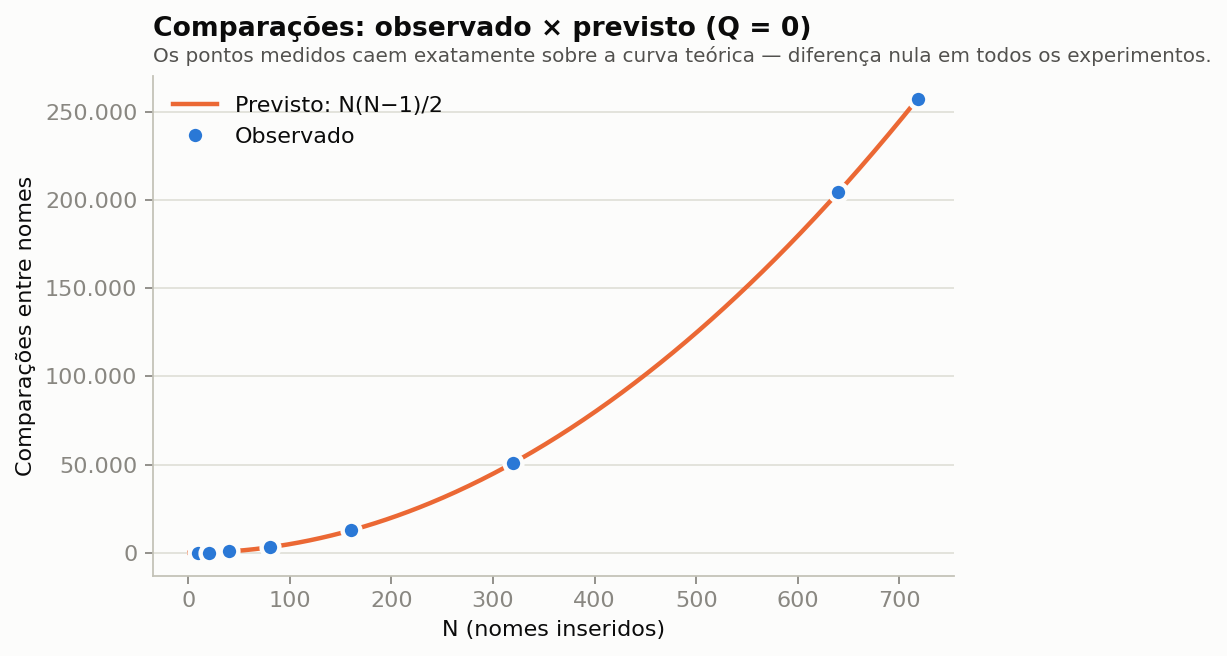
\includegraphics[width=\textwidth]{../graficos/g1_observado_previsto.png}
\caption{Comparações observadas (pontos) sobre a curva teórica $\frac{N(N-1)}{2}$ (linha). Não há ponto fora da curva: a sobreposição é exata, não aproximada.}
\end{figure}

\begin{figure}[H]
\centering
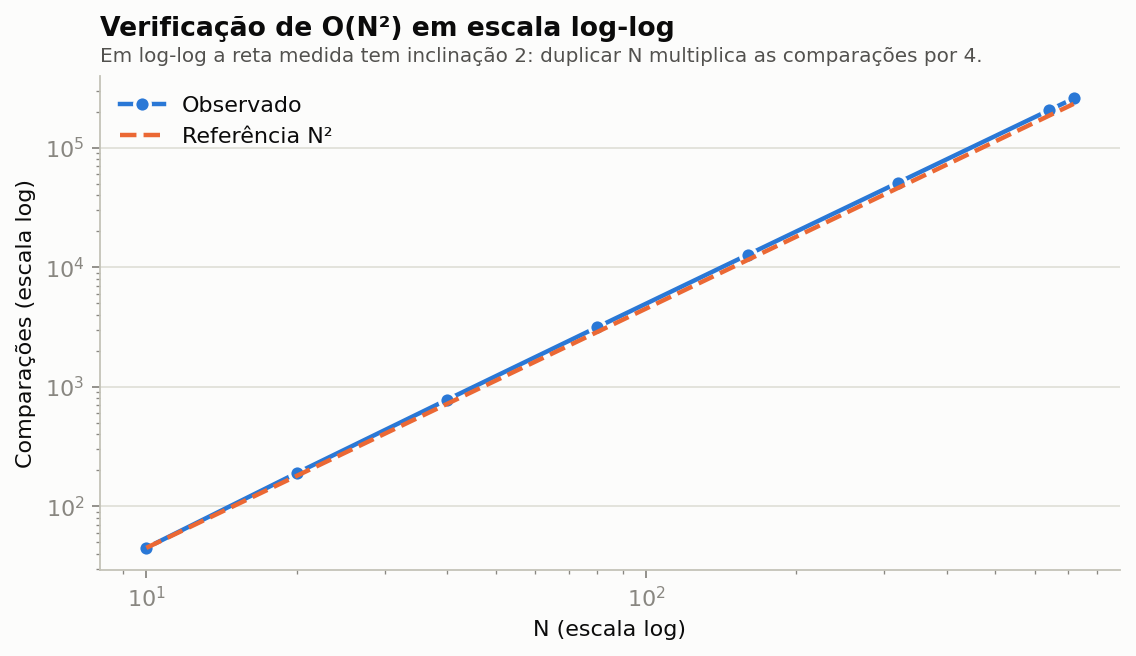
\includegraphics[width=\textwidth]{../graficos/g2_loglog.png}
\caption{Os mesmos dados em escala log-log. Uma função potência $N^{a}$ aparece como reta de inclinação $a$ neste tipo de gráfico; o ajuste por mínimos quadrados sobre os dados medidos resulta em inclinação $2{,}0198$, coerente com $\Theta(N^2)$.}
\label{fig:loglog}
\end{figure}

\begin{figure}[H]
\centering
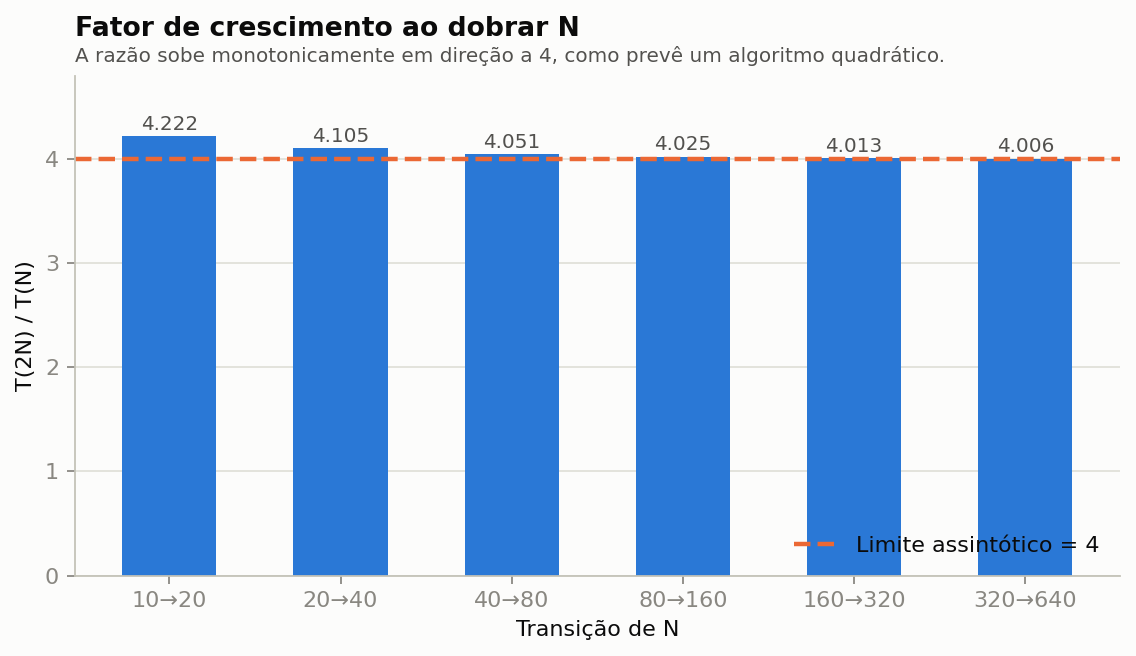
\includegraphics[width=\textwidth]{../graficos/g3_dobrar_n.png}
\caption{Razão $T(2N)/T(N)$ medida em cada duplicação de $N$. A razão decresce monotonicamente em direção a 4, aproximando-se por cima, exatamente como prevê a Equação~\eqref{eq:razao}.}
\label{fig:dobrar}
\end{figure}

\begin{figure}[H]
\centering
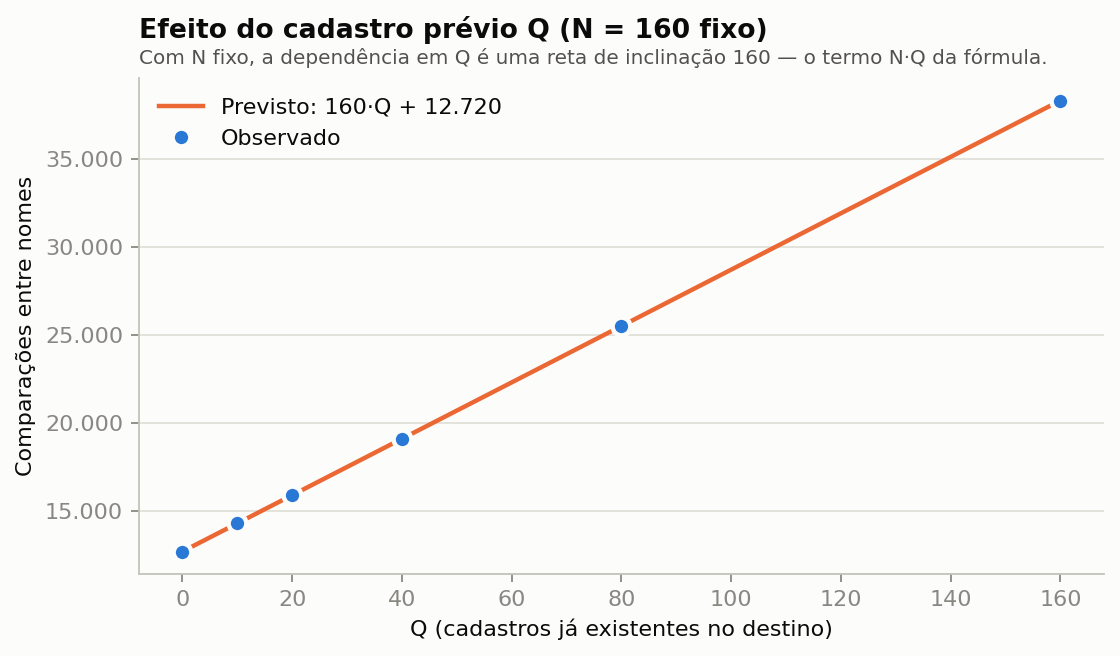
\includegraphics[width=\textwidth]{../graficos/g4_termo_nq.png}
\caption{Experimento C. Com $N=160$ fixo, as comparações crescem linearmente com $Q$, sobre a reta $160Q + 12.720$ --- confirmação direta do termo $N \cdot Q$ da fórmula.}
\label{fig:nq}
\end{figure}

\newpage

\clearpage
\subsection{Experimentos D e E: fora da hipótese de nomes distintos}

\begin{table}[H]
\centering
\small
\begin{tabular}{lrrrr}
\toprule
\textbf{Experimento} & \textbf{Registros lidos} & \textbf{Inseridos} & \textbf{Redundantes} & \textbf{Comparações} \\
\midrule
D --- arquivo completo, $Q=0$   & 719 & 718 & 1   & 257.841 \\
E --- reexecução, $Q=718$       & 719 & 0   & 719 & 258.559 \\
\bottomrule
\end{tabular}
\caption{Experimentos com redundâncias reais. Note que o Experimento D insere os mesmos 718 nomes do último ponto do Experimento A, mas registra 438 comparações a mais.}
\label{tab:de}
\end{table}

Saída do Experimento D (trecho final):

\begin{lstlisting}[style=terminal]
ERRO: nome redundante encontrado: MARCELO MACHADO VIANA

Registros lidos na origem   : 719
Cadastros previos no destino: 0
Nomes inseridos             : 718
Nomes redundantes           : 1
Comparacoes entre nomes     : 257841
\end{lstlisting}

% ------------------------------------------------------------------ 10
\section{Comparação entre os resultados teóricos e empíricos}
\label{sec:comparacao}

\subsection{Aderência quantitativa}

Nos Experimentos A, B e C --- as 22 execuções em que a hipótese (H2) é satisfeita --- a diferença entre observado e previsto foi \textbf{zero em todos os pontos}, sem exceção. Não se trata de uma aproximação com erro pequeno, mas de coincidência exata dígito a dígito, inclusive em valores da ordem de $2{,}5 \times 10^5$ comparações.

Três aspectos distintos da fórmula foram testados separadamente, e cada um se confirmou:

\begin{itemize}[leftmargin=1.4em,itemsep=3pt]
  \item o \textbf{termo quadrático} $\frac{N(N-1)}{2}$, pelo Experimento A, variando $N$ ao longo de quase duas ordens de grandeza;
  \item o \textbf{termo linear} $N \cdot Q$, pelo Experimento C, que mantém $N$ fixo e varia $Q$: cada acréscimo de 10 cadastros prévios produziu exatamente 1.600 comparações adicionais, isto é, $160 \times 10$ (Tabela~\ref{tab:c} e Figura~\ref{fig:nq});
  \item a \textbf{combinação dos dois}, pelo Experimento B.
\end{itemize}

Testar os termos em separado é metodologicamente relevante: uma fórmula pode reproduzir bem os dados por compensação entre parcelas erradas. Variando um parâmetro por vez, essa possibilidade é descartada.

\subsection{O exemplo do enunciado como caso particular $Q=1$}

Um resultado merece destaque. O ``Exemplo de saída'' fornecido no enunciado é:

\begin{lstlisting}[style=terminal]
nomes_inseridos,comparacoes
10,55
20,210
40,820
80,3240
160,12880
\end{lstlisting}

Esses valores \emph{não} correspondem a $\frac{N(N-1)}{2}$, que daria 45, 190, 780, 3.160 e 12.720. Eles correspondem a $\frac{N(N+1)}{2}$. Pela Equação~\eqref{eq:q1}, essa é precisamente a especialização de $T(N,Q)$ em $Q = 1$:

\[
T(N,1) \;=\; N \cdot 1 + \frac{N(N-1)}{2} \;=\; \frac{N(N+1)}{2}.
\]

O Experimento B reproduziu esses cinco números exatamente (Tabela~\ref{tab:b}), bastando iniciar o destino com um cadastro prévio. Trata-se, portanto, de uma evidência particularmente forte a favor do modelo: a fórmula geral não apenas descreve os dados coletados por este trabalho, mas também \emph{prevê} o conjunto de valores fornecido independentemente no enunciado, identificando ao mesmo tempo a condição experimental que o gera.

\subsection{Taxa de crescimento ao dobrar $N$}

A Tabela~\ref{tab:razoes} confronta as razões medidas com as previstas pela Equação~\eqref{eq:razao}.

\begin{table}[H]
\centering
\small
\begin{tabular}{lrrr}
\toprule
\textbf{Transição} & \textbf{Razão medida} & \textbf{Previsto por $\frac{4N-2}{N-1}$} & \textbf{Diferença} \\
\midrule
$10 \to 20$   & 4,2222 & 4,2222 & 0,0000 \\
$20 \to 40$   & 4,1053 & 4,1053 & 0,0000 \\
$40 \to 80$   & 4,0513 & 4,0513 & 0,0000 \\
$80 \to 160$  & 4,0253 & 4,0253 & 0,0000 \\
$160 \to 320$ & 4,0126 & 4,0126 & 0,0000 \\
$320 \to 640$ & 4,0063 & 4,0063 & 0,0000 \\
\bottomrule
\end{tabular}
\caption{Fator de crescimento observado ao dobrar $N$, comparado ao valor exato previsto. A razão converge para 4 por cima, e o desvio em relação a 4 cai pela metade a cada duplicação.}
\label{tab:razoes}
\end{table}

A concordância é total, e o padrão de convergência também é o previsto: a razão nunca é exatamente 4 para $N$ finito, aproxima-se de 4 por valores maiores, e a distância até 4 --- que vale $\frac{2}{N-1}$ --- reduz-se pela metade a cada duplicação de $N$. Os valores medidos seguem esse comportamento: $0{,}2222$, $0{,}1053$, $0{,}0513$, $0{,}0253$, $0{,}0126$, $0{,}0063$.

\subsection{O desvio do Experimento D, e por que ele é esperado}

O Experimento D é o único em que observado e previsto divergem, e isso não enfraquece o modelo --- ao contrário, delimita com precisão o seu domínio de validade. Comparando com o último ponto do Experimento A, que insere os mesmos 718 nomes:

\[
257.841 \;-\; 257.403 \;=\; 438.
\]

O desvio é explicado integralmente. O arquivo completo tem 719 registros, dos quais 718 são inserções e um é redundante. As 718 inserções custam, pela fórmula, $\frac{718 \times 717}{2} = 257.403$ comparações. Resta o custo da busca pelo registro redundante: \texttt{MARCELO MACHADO VIANA} foi inserido como o 438\textsuperscript{o} nome do vetor, e a busca sequencial \emph{interrompe-se ao encontrar} a igualdade, consumindo 438 comparações em vez de percorrer as 705 posições existentes naquele momento. Logo:

\[
257.403 \;+\; 438 \;=\; 257.841,
\]

\noindent exatamente o valor medido. O modelo, estendido para contemplar buscas bem-sucedidas, continua exato; o que a fórmula original não cobre é apenas o caso excluído por hipótese.

O Experimento E confirma a mesma mecânica em regime extremo. Com o destino contendo os 718 nomes e nenhuma inserção possível, cada uma das 719 buscas é bem-sucedida e termina na posição em que o nome está armazenado. Como esses nomes ocupam as posições 1 a 718 na mesma ordem do arquivo, o total previsto é

\[
\sum_{i=1}^{718} i \;+\; 438 \;=\; 258.121 + 438 \;=\; 258.559,
\]

\noindent que é precisamente o valor medido. Vale notar que $\frac{718+1}{2} = 359{,}5$ comparações por busca corresponde ao custo médio conhecido da busca sequencial bem-sucedida com posições uniformemente distribuídas --- resultado clássico que aqui aparece como consequência aritmética, e não como estimativa.

% ------------------------------------------------------------------ 11
\section{Discussão dos resultados}
\label{sec:discussao}

Esta seção responde diretamente às questões propostas na Parte 4 do enunciado.

\subsection*{1. Os dados empíricos confirmam a hipótese de complexidade temporal proposta?}

Sim, e de forma incomumente categórica. Em 22 execuções sob as hipóteses da análise, a diferença entre previsto e medido foi zero em todas. Além da aderência pontual, a \emph{forma} do crescimento também se confirma: a inclinação do ajuste log-log é $2{,}0198$ (Figura~\ref{fig:loglog}) e a razão $T(2N)/T(N)$ converge para 4 (Figura~\ref{fig:dobrar}), ambas assinaturas de crescimento quadrático. Os dados confirmam a hipótese $\Theta(N^2)$.

\subsection*{2. Como a taxa de crescimento observada se comporta quando a quantidade de nomes dobra?}

O número de comparações \textbf{aproximadamente quadruplica}, e o desvio em relação ao fator 4 é ele mesmo previsível. As razões medidas foram $4{,}2222$, $4{,}1053$, $4{,}0513$, $4{,}0253$, $4{,}0126$ e $4{,}0063$ --- estritamente decrescentes, sempre acima de 4, com a distância até 4 caindo pela metade a cada duplicação. Isso é exatamente $\frac{4N-2}{N-1} = 4 + \frac{2}{N-1}$. O fator 4 não é um valor aproximado obtido por ajuste: é o limite de uma expressão fechada, e os dados seguem a expressão inteira, não apenas o seu limite.

\subsection*{3. Existem diferenças entre os valores teóricos e os valores medidos? Em caso afirmativo, explique suas possíveis causas.}

Nos Experimentos A, B e C não há diferença alguma. Isso pode surpreender quem esteja habituado a validações experimentais de desempenho, e a razão está na natureza da grandeza medida. O contador registra um \textbf{evento discreto do algoritmo} --- cada execução de \texttt{strcmp} dentro do laço de busca --- e não um intervalo de tempo. Não há, portanto, as fontes usuais de ruído: nada de escalonamento de processos, hierarquia de \emph{cache}, frequência variável de processador, coleta de lixo ou resolução de relógio. O contador mede a mesma quantidade que a análise combinatória calcula. Duas execuções idênticas produzem o mesmo número, e o modelo, se correto, deve acertar exatamente. Foi o que ocorreu.

Há diferença, sim, no Experimento D: 438 comparações acima do previsto. A causa é a \emph{violação deliberada da hipótese} (H2), e não um erro do modelo nem imprecisão de medida. A fórmula $NQ + \frac{N(N-1)}{2}$ pressupõe que toda busca seja malsucedida e percorra o vetor completo. Quando existe um nome repetido, a busca correspondente termina antecipadamente, no ponto em que a igualdade é encontrada. Como se mostrou na Seção~\ref{sec:comparacao}, o desvio de 438 é exatamente a posição em que o nome repetido estava armazenado, e a soma $257.403 + 438$ reproduz o valor medido sem resíduo.

Vale registrar que essa é uma diferença \emph{para cima}, o que pode parecer contraintuitivo, já que uma busca interrompida é mais barata. A explicação é que o Experimento D processa 719 registros e não 718: o registro extra acrescenta uma busca que a fórmula, calculada para $N = 718$ inserções, não contabiliza.

Uma causa potencial de divergência que convém mencionar, embora não tenha se materializado aqui, é a \textbf{ordem dos registros}. Sob (H2) a ordem é irrelevante --- todas as buscas são completas, independentemente de como os nomes estejam dispostos. Quando há redundâncias, a ordem passa a importar: se o nome repetido estivesse no início do vetor em vez da posição 438, o desvio seria proporcionalmente menor.

\subsection*{4. Os resultados experimentais sustentam a demonstração matemática apresentada?}

Sustentam, com a ressalva epistemológica de que experimentos não demonstram teoremas. A prova por indução estabelece a fórmula para todo $N \geq 1$ por dedução lógica, e é ela que garante a generalidade do resultado; os experimentos não poderiam fazê-lo, pois cobrem um número finito de casos.

O que os experimentos fazem é validar as duas coisas que a demonstração \emph{pressupõe}: que a modelagem do custo de cada inserção está correta, e que o programa implementado é de fato o algoritmo analisado. O passo indutivo afirma que a $(k{+}1)$-ésima inserção custa $Q + k$ comparações. O Experimento C é o teste direto dessa afirmação: mantendo $N$ fixo e variando $Q$, o custo variou linearmente com inclinação exatamente 160, como o termo $Q$ da recorrência exige. E o encaixe perfeito em todos os valores de $N$ mostra que a recorrência acumulada não perde nada pelo caminho. Uma divergência nos dados apontaria erro na modelagem ou na implementação --- e nenhuma apareceu.

\subsection*{5. Qual é a evidência empírica de que o algoritmo possui a complexidade temporal indicada pela análise teórica?}

A evidência se organiza em quatro níveis, de robustez crescente:

\begin{enumerate}[leftmargin=1.6em,itemsep=3pt]
  \item \textbf{Aderência exata da fórmula fechada.} Diferença nula nos 22 pontos, em três desenhos experimentais distintos, com $N$ variando de 10 a 718 e $Q$ de 0 a 160.
  \item \textbf{Inclinação log-log igual a 2.} O ajuste linear de $\log T$ contra $\log N$ resultou em $2{,}0198$. Uma função linear daria inclinação 1; uma cúbica, 3. O pequeno excesso sobre 2 é explicado: o termo $-\frac{N}{2}$ da fórmula torna a curva ligeiramente subquadrática para $N$ pequeno, o que enviesa o ajuste para cima quando os pontos menores são incluídos.
  \item \textbf{Quadruplicação ao dobrar $N$.} Esta é a evidência mais importante do ponto de vista assintótico, porque não depende de constantes multiplicativas: qualquer algoritmo $\Theta(N^2)$ exibe razão tendendo a 4, e nenhum algoritmo de outra ordem o faz --- linear tenderia a 2, cúbico a 8. A razão medida cai de $4{,}2222$ para $4{,}0063$ ao longo das seis duplicações.
  \item \textbf{Decomposição confirmada termo a termo.} O Experimento C confirma o termo $N \cdot Q$ isoladamente, mostrando que a fórmula está certa em sua estrutura, e não apenas em seus valores agregados.
\end{enumerate}

\subsection*{6. Comparação explícita entre os dados observados e a hipótese formulada}

A hipótese formulada foi: \emph{o número de comparações entre nomes é dado por $T(N,Q) = N \cdot Q + \frac{N(N-1)}{2}$, e portanto o algoritmo é $\Theta(N^2)$.}

Os resultados \textbf{fortalecem} essa hipótese, pelas seguintes razões:

\begin{itemize}[leftmargin=1.4em,itemsep=3pt]
  \item a hipótese faz \emph{previsões pontuais exatas}, não apenas afirmações sobre tendências. Uma previsão exata é altamente falsificável: qualquer erro de modelagem apareceria imediatamente como diferença não nula. Vinte e duas oportunidades de falsificação foram oferecidas, e nenhuma se concretizou;
  \item a hipótese foi testada em seus componentes separadamente, e cada componente se confirmou por variação independente do parâmetro correspondente;
  \item a hipótese \emph{previu corretamente dados que não foram gerados por este trabalho} --- os cinco valores do exemplo do enunciado --- e identificou a condição ($Q = 1$) que os produz. Prever dados externos é evidência mais forte que descrever dados próprios;
  \item o único desvio observado ocorreu onde a própria hipótese declara não se aplicar, e foi quantitativamente explicado até a última unidade. Uma hipótese que também acerta o tamanho do seu próprio erro nas condições de contorno é mais forte, e não mais fraca, do que uma que apenas acerta no domínio confortável.
\end{itemize}

Não se identificou nenhuma evidência que enfraqueça a hipótese.

\subsection*{Implicação prática}

Cabe uma observação sobre a natureza do algoritmo. A classificação $\Theta(N^2)$ não é uma curiosidade teórica: ela diz que o serviço não escala. Para os 718 nomes deste arquivo, 257.403 comparações são irrelevantes --- a execução é instantânea. Mas o custo cresce com o quadrado: um cadastro de 100.000 bolsistas exigiria cerca de $5 \times 10^9$ comparações de cadeias de caracteres, e 1.000.000 de bolsistas levariam a $5 \times 10^{11}$ --- inviável na prática.

O gargalo está na estrutura de dados, não na linguagem nem na máquina. Substituir o vetor com busca sequencial por uma tabela de dispersão reduziria o custo esperado de verificação a $O(1)$ por registro e o total a $O(N + Q)$; uma árvore de busca balanceada daria $O((N+Q)\log(N+Q))$. Para o cenário descrito no enunciado --- um serviço que recebe solicitações continuamente por uma API e as incorpora a um cadastro que só cresce --- essa troca é a diferença entre um sistema que funciona e um que degrada a cada registro adicionado.

% ------------------------------------------------------------------ 12
\section{Conclusão}

O trabalho implementou em C o serviço de importação de bolsistas com detecção de redundância por busca sequencial, instrumentou o algoritmo com um contador de comparações e conduziu uma análise que relaciona quatro elementos: a função deduzida, a demonstração formal, os dados medidos e a classificação assintótica.

A \textbf{função matemática deduzida} foi $T(N,Q) = N \cdot Q + \frac{N(N-1)}{2}$, obtida somando os custos individuais das $N$ inserções, cada uma delas percorrendo um vetor de $Q + i - 1$ nomes. Seus dois termos têm significado próprio: $N \cdot Q$ é o custo de confrontar os nomes novos com o cadastro preexistente, e $\frac{N(N-1)}{2} = \binom{N}{2}$ é o custo de confrontar os nomes novos entre si, um por par.

A \textbf{demonstração por indução} estabeleceu essa fórmula para todo $N \geq 1$. O caso base $N = 1$ fornece $Q$ comparações, coincidente com a fórmula; o passo indutivo acrescenta ao custo de $k$ nomes as $Q + k$ comparações da $(k{+}1)$-ésima inserção e recupera algebricamente a mesma expressão em $k+1$. A prova também explicita a fronteira do resultado: ele vale sob a hipótese de nomes distintos, que é o que garante que toda busca seja malsucedida e completa.

Os \textbf{dados coletados} confirmaram a fórmula sem nenhuma margem de erro. Nas 22 execuções realizadas sob a hipótese de distinção, a diferença entre observado e previsto foi zero em todos os pontos, para $N$ entre 10 e 718 e $Q$ entre 0 e 160. Os termos quadrático e linear foram validados separadamente, e a fórmula reproduziu o exemplo de saída do próprio enunciado como o caso particular $Q = 1$. A única divergência observada, no experimento com o arquivo completo, decorre da redundância real ali presente e foi explicada exatamente pelo encerramento antecipado da busca na posição 438.

A \textbf{classificação assintótica} é $T(N) = \Theta(N^2)$, e portanto $O(N^2)$, para $Q$ constante --- e permanece $\Theta(N^2)$ mesmo se $Q$ crescer proporcionalmente a $N$. A evidência empírica dessa classificação é independente das constantes envolvidas: ao dobrar $N$, as comparações se multiplicam por um fator que caiu de $4{,}2222$ para $4{,}0063$ ao longo de seis duplicações, convergindo para 4 conforme a expressão exata $4 + \frac{2}{N-1}$; e o ajuste log-log tem inclinação $2{,}02$.

Quanto à \textbf{validade da hipótese à luz das evidências}, a conclusão do grupo é que as evidências a fortalecem. A hipótese arriscou previsões numéricas exatas em vez de tendências, foi testada termo a termo por variação independente dos parâmetros, acertou um conjunto de dados fornecido externamente, e delimitou corretamente o seu próprio domínio de validade --- inclusive prevendo a magnitude do desvio no caso excluído. Nenhuma evidência contrária foi encontrada.

A lição de engenharia que fica é que o algoritmo está correto e é inadequado ao mesmo tempo. Ele resolve o problema especificado e não escala: o custo por registro inserido cresce linearmente com o tamanho do cadastro, de modo que o serviço fica mais lento a cada bolsista cadastrado. A análise quantifica esse limite e indica onde intervir --- na estrutura de dados que sustenta a verificação de redundância.

% ------------------------------------------------------------------ repo
\section{Repositório Git}

Todo o material deste trabalho está versionado em repositório Git público:

\begin{center}
\fbox{\parbox{0.9\textwidth}{\centering\ttfamily\url{\repositorio}}}
\end{center}

\noindent O repositório contém:

\begin{itemize}[leftmargin=1.4em,itemsep=2pt]
  \item \texttt{src/copiador.c} --- código-fonte completo do programa em C;
  \item \texttt{dados/bolsistas-2025.csv} --- arquivo de entrada original;
  \item \texttt{experimentos/entradas/} --- recortes utilizados nos testes;
  \item \texttt{experimentos/estatisticas/} --- arquivos CSV gerados nos experimentos;
  \item \texttt{experimentos/destinos/} e \texttt{experimentos/saidas/} --- arquivos de destino e saídas padrão produzidas pelo programa;
  \item \texttt{Makefile} e \texttt{rodar\_experimentos.sh} --- compilação e execução da bateria completa;
  \item \texttt{analisar.py} --- confronto com o modelo teórico e geração dos gráficos;
  \item \texttt{README.md} --- instruções de compilação e de execução;
  \item \texttt{relatorio/} --- fonte deste relatório.
\end{itemize}

\subsection*{Compilação}

\begin{lstlisting}[style=terminal]
make
# ou, sem o Makefile:
gcc -O2 -Wall -Wextra -std=c99 -o src/copiador src/copiador.c
\end{lstlisting}

\subsection*{Execução}

\begin{lstlisting}[style=terminal]
./src/copiador dados/bolsistas-2025.csv cadastro.csv estatisticas.csv
\end{lstlisting}

\subsection*{Reprodução dos experimentos}

\begin{lstlisting}[style=terminal]
./rodar_experimentos.sh     # compila e executa as 24 execucoes
python3 analisar.py         # tabelas e graficos
\end{lstlisting}

% ------------------------------------------------------------------ apendice
\appendix
\section{Código-fonte completo}

\lstinputlisting[style=c]{../src/copiador.c}

\end{document}
